\section{RQ1: Reddit Misinformation Submissions vs Authentic News Submissions}\label{sec:rq1}
Having outlined our methodology, in this section we turn to understand the relative levels of toxicity and polarization orientations of users and subreddits that interact with misinformation and authentic news. 




%\subsection{Misinformation vs Mainstream Submissions}


\subsection{Experimental Setup}
As previously mentioned, on Reddit, users can submit news articles from different websites as a submission under which users can comment and discuss the article or issues prompted by the news article headline. To understand the relative presence of political incivility and toxic comments compelled by misinformation, we thus first compare levels of toxic comments posted under misinformation and authentic news URL submissions.

To do this, across all our collected subreddits we gather the sets the URL submissions that utilize our set of misinformation and authentic news websites. Altogether, within our Pushshift dataset, there were 38,264 different submissions utilizing our first set of 541 misinformation websites from 2,217 different subreddits and 226,930 submissions utilizing our first set of 565 authentic news websites from 18,383 unique subreddits. This difference in magnitude of submissions, we believe, is largely due to the greater popularity and widespread appeal of authentic mainstream news compared with alternative and more fringe websites. Indeed, utilizing the Amazon Alexa Top Million list from March 1, 2021~\cite{amazon-top-mil}, we find that 255 authentic news websites were in the top 100K websites, while only 101 misinformation websites were in the top 100K. To further bolster and confirm our results, we test our findings in this section utilizing our second set of misinformation and mainstream websites. Altogether, from this second set of URLs, we find an additional set of 9,558 misinformation and 560,673 authentic news submissions.

\subsection{Differences in Toxicity/Incivility between Misinformation and Authentic News Submissions}\label{sec:toxicity}

Looking at the toxicity comments from our first set of misinformation domains, we see that 14.9\% of the submission had at least one toxic comment and 1.35\% of all the comments were toxic. In contrast, for the first set of authentic submissions 13.6\% of the submissions had a toxic comment and only 0.85\% of the comments were toxic. We thus see a 60\% uptick in the rate at which toxic comments are posted on the misinformation submissions. Confirming this finding with our second set of 9,558 misinformation and 560,673 authentic news submissions, we again see a similar pattern of higher toxicity in the misinformation submission comments. 15.3\% of the misinformation submissions had toxic comments with 0.92\% of the comments being toxic. In contrast, 11.74\% of the mainstream submissions had toxic comments with 0.64\% of the comments being toxic. We thus see in this replicated experiment that Reddit misinformation conversations indeed have a higher incidence and occurrence of toxicity and incivility. Putting all these conversations together, we find that 1.17\% of comments under misinformation submissions are toxic/uncivil while 0.7\% of comments for authentic news websites are toxic/uncivil. we thus find an overall 63\% increase in the rate at which toxic comments are posted on misinformation submissions.

\begin{figure*}
\begin{subfigure}{.4\textwidth}
  \centering
  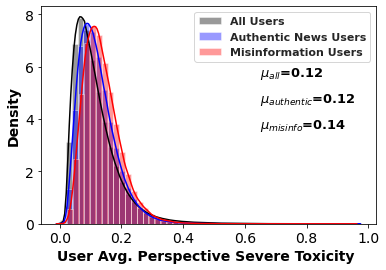
\includegraphics[width=1\linewidth]{figures/user_toxicity_above10.png}
  \caption{URL Set 1}
\label{fig:harmonic-sub1}
\end{subfigure}
\begin{subfigure}{.4\textwidth}
  \centering
  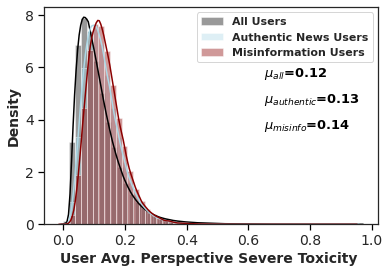
\includegraphics[width=1\linewidth]{figures/user_toxicity_above10_2.png}
    \caption{URL Set 2}
  \label{fig:pagerank-sub2}
\end{subfigure}

\caption{\textbf{Toxicity levels for users who comment under authentic News and misinformation URL Reddit submissions}---Users who interact with misinformation submissions are slightly more toxic/uncivil than users that interact with authentic news. Both groups are slightly more toxic/uncivil than Reddit users generally. }
\label{fig:users-misinformation-authentic-toxicity}
\end{figure*}
%\paragraph{User and Subreddit Toxicity in Misinformation and Mainstream Reddit Submissions }
%  We now seek to eke out some of the causes the higher amount of toxicity within the misinformation URL submissions on Reddit. 


Higher toxicity within misinformation submissions could be caused by (1) more toxic/uncivil users participating in these conversations or (2) higher toxicity norms in the subreddits where the misinformation was posted. As seen in Figure~\ref{fig:users-misinformation-authentic-toxicity}, we see that these users are slightly more toxic than their authentic news counterparts. For the first group of URL submissions, on average 1.54\% of the comments for the users associated with these submissions are toxic/uncivil compared with 1.22\% for the corresponding group of authentic news users. Similarly, on average 1.48\% of comments posted by the second group of misinformation users are toxic compared to 1.32\% for the authentic news commenters. However, for bot URL groups, as seen in Figure~\ref{fig:users-misinformation-authentic-toxicity}, the distributions of their Perspective API scores are fairly close. We note, that despite this proximity in toxicity of misinformation commenters between authentic news commenters, the higher user toxicity appears stable even among users from the same subreddits. Comparing the users who posted in subreddits where \emph{both} mainstream and misinformation URLs were posted, we still see that the users who posted on misinformation submissions had elevated rates of toxicity (1.21\% compared to 1.45\%). We thus see ``more toxic'' users are indeed commenting more on misinformation submissions compared to authentic news submissions. Finally, to further confirm our results, we perform U-Mann Whitney tests to ensure that there are indeed statistically significant differences between the rate of toxicity in misinformation and authentic news users; running these tests finding p-values $<10^{-12}$, we indeed conclude that both groups URL submission commenters that there are indeed higher rates of toxicity for the misinformation users.

However, despite the finding that more toxic users are indeed commenting more often on misinformation submissions, their higher rate of toxicity is not enough to explain the larger amount of toxic comments in misinformation submissions. After accounting for the higher rate of user toxicity across all the URL submissions, we still see 25.4\% more toxic comments than would be expected for the first set of URLs and 28.0\% for the second comparison set. Other factors, besides the specific users that comment on misinformation, are contributing to the higher rate of toxicity on misinformation submissions.



\begin{figure*}
\begin{subfigure}{.4\textwidth}
  \centering
  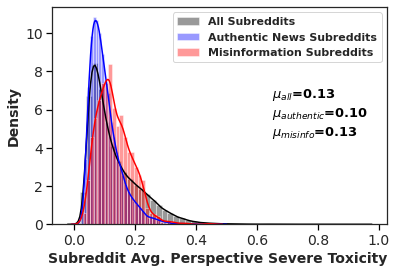
\includegraphics[width=1\linewidth]{figures/subreddit_toxicity_above10.png}
      \caption{URL Set 1}
\label{fig:harmonic-sub1}
\end{subfigure}%s
\begin{subfigure}{.4\textwidth}
  \centering
  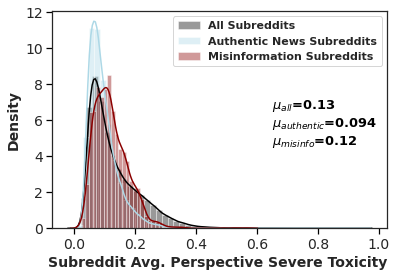
\includegraphics[width=1\linewidth]{figures/subreddit_toxicity_above10_2.png}
      \caption{URL Set 2}
  \label{fig:pagerank-sub2}
\end{subfigure}

\caption{\textbf{Toxicity Levels in Subreddits with Authentic News and Misinformation URL Submission}---Subreddits with misinformation submissions are overall more toxic/uncivil compared with authentic news subreddits and subreddits more generally.}
\label{fig:subreddit-misinformation-authentic-toxicity}
\end{figure*}

Looking at the role of subreddits in promoting toxicity in Figure~\ref{fig:subreddit-misinformation-authentic-toxicity}, we find that the toxicity norms of subreddits with misinformation submissions also contribute to higher levels of toxic comments. We see that on average for both sets of URLs that we consider, the set of subreddits with misinformation submissions have higher levels of toxicity compared to subreddits with authentic news submissions. Altogether, in our first set of misinformation URLs, for corresponding subreddits 1.40\% of comments posted there are toxic/uncivil. This is compared to a corresponding rate of 0.80\% for comments within subreddits with authentic news submissions. We see a similar difference from our second set of URLs (1.1\% vs 0.7\%). From these two datasets, we thus find that users in subreddits with misinformation submissions post toxic comments at a rate between 57\% (second set of URLs) and 75\% (first set of URLs) higher than in subreddits with authentic news submissions. We again perform U-Mann Whitney tests to ensure that there are indeed statistically significant differences between the rate of toxicity in misinformation and authentic news subreddits. With p-values $<10^{-12}$, we conclude that for both groups that there are indeed higher levels of toxicity in the misinformation subreddits.

\subsection{Differences in Political Polarization between Misinformation and Authentic News Submissions}\label{sec:polarization}
Having seen the higher levels of toxicity/incivility present within misinformation Reddit submissions, we now explore the differences in political polarization between users who comment on misinformation and those that comment on authentic news.

\begin{figure*}
\begin{subfigure}{.4\textwidth}
  \centering
  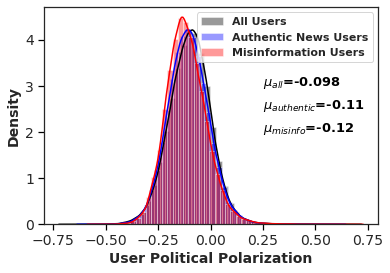
\includegraphics[width=1\linewidth]{figures/user_political_comparison.png}
      \caption{URL Set 1}
\label{fig:political-users1}
\end{subfigure}%s
\begin{subfigure}{.4\textwidth}
  \centering
  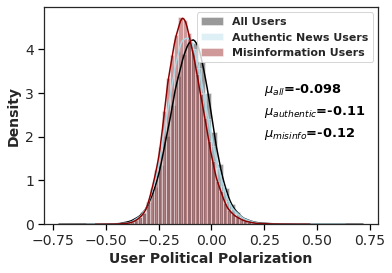
\includegraphics[width=1\linewidth]{figures/user_political_comparison2.png}
      \caption{URL Set 2}
  \label{fig:political-users2}
\end{subfigure}

\caption{\textbf{Political polarization of users who comment under authentic news and misinformation Reddit submissions}-- There are not significant differences in political ideology between users who comment on misinformation and those that comment on authentic news. }
\label{fig:users-political-orientation}
\end{figure*}
\begin{figure*}
\begin{subfigure}{.4\textwidth}
  \centering
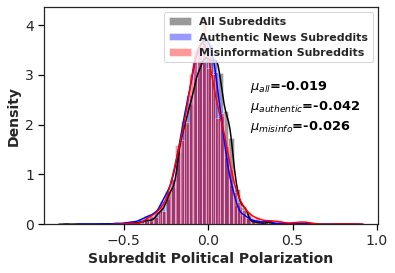
\includegraphics[width=1\linewidth]{figures/subreddit_political_comparison.png}
    \caption{URL Set 1}
\label{fig:harmonic-sub1}
\end{subfigure}%s
\begin{subfigure}{.4\textwidth}
  \centering
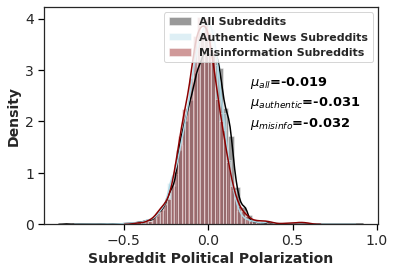
\includegraphics[width=1\linewidth]{figures/subreddit_political_comparison2.png}
    \caption{URL Set 2}
  \label{fig:pagerank-sub2}
\end{subfigure}

\caption{\textbf{Political polarization of subreddits with authentic news and misinformation Reddit submissions}--- There are no significant differences in the political orientation of subreddits where misinformation and authentic news appear. }
\label{fig:subreddit-misinformation-authentic-toxicity}
\end{figure*}
Looking at the set of users commenting under misinformation Reddit submissions, we surprisingly do not see dramatic differences between these users and those that comment on authentic news submissions. In fact, as seen in Figure~\ref{fig:users-political-orientation} for both our set of misinformation URL sets, we see a slight leftward tilt in the average commenter. Similarly and surprisingly, looking in Figure~\ref{fig:subreddit-misinformation-authentic-toxicity} at the political orientation of the subreddits where our misinformation submissions appeared, we again see that there is not much difference in their respective polarizations. This appears to indicate that \emph{both} misinformation and authentic news appear within subreddits and get commented on by users across the political spectrum.

%This indicates that the particular higher levels of toxicity observed in our set of misinformation-filled subreddits is not being driven by the political environment of the subreddit. 

We note that despite misinformation appearing in subreddits across the political spectrum, the users that post misinformation have a rightward tilt compared to the users that comment on misinformation. As seen in Figure~\ref{figure:misinformation-posters-commenters}, for both sets of URLs submissions with comments, we see that misinformation submitters are on the whole more conservative than their corresponding more liberal commenters. This is largely in contrast to authentic news commenters and posters. As seen in Figure~\ref{figure:news-posters-commenters}, authentic news posters and commenters share nearly the exact same distribution. 




\begin{figure}
\centering
\begin{subfigure}{.4\textwidth}
  \centering
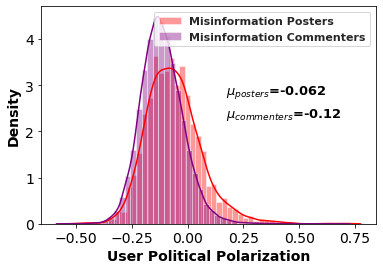
\includegraphics[width=1\linewidth]{figures/misinformation_posters_commenters.png}
    \caption{URL Set 1}
\end{subfigure}
\begin{subfigure}{.4\textwidth}
  \centering
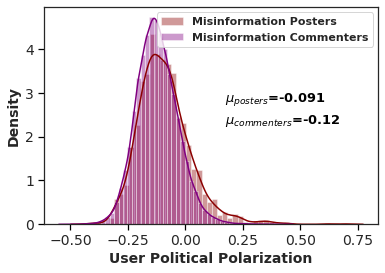
\includegraphics[width=1\linewidth]{figures/misinformation_posters_commenters2.png}
    \caption{URL Set 2}
\end{subfigure}
\caption{\textbf{Distribution of political orientation of posters and commenters of misinformation}--- There is a noticeable rightward tilt in users that post misinformation compared to those that comment on misinformation.}
\label{figure:misinformation-posters-commenters}

\end{figure}



\begin{figure}
\centering
\begin{subfigure}{.4\textwidth}
  \centering
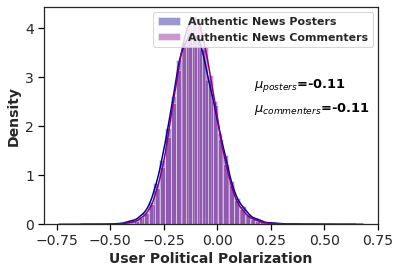
\includegraphics[width=1\linewidth]{figures/news_posters_comenters_comparison.png}
    \caption{URL Set 1}
\end{subfigure}
\begin{subfigure}{.4\textwidth}
  \centering
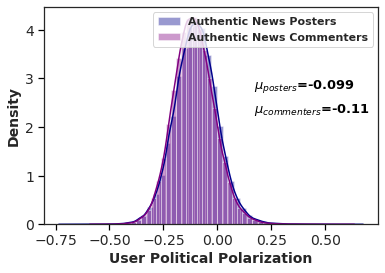
\includegraphics[width=1\linewidth]{figures/news_posters_comenters_comparison2.png}
    \caption{URL Set 2}
\end{subfigure}
\caption{\textbf{Distribution of political orientation of posters and commenters of authentic news}--- Unlike for misinformation posts, the posters and the commenters on authentic news share similar distributions of political orientations.}
\label{figure:news-posters-commenters}
\end{figure}

Altogether, we thus observe (especially in contrast to authentic news submissions), that a politically different set of users post misinformation news compared to those that comment on it. While we did not observe that the polarization levels of users who comment on misinformation are substantially different from commenters on authentic users, we did observe that they \emph{are} different from posters of misinformation content. 

\subsection{Intersection of Misinformation, News Media, Toxicity, and Political Polarization across Subreddits}
Finally, having seen the distribution of the political polarization and toxicity among different users and in different environments, we now look if these different characteristics correlate with the amount of misinformation and authentic news in each subreddit. Namely, we seek to determine more broadly if levels of misinformation are correlated with increased levels of toxicity. To do this we rely on our list of \textit{misinfo-oriented} and \textit{mainstream-oriented} websites.



Specifically, for each subreddit in our dataset, we compute their \textit{misinformation similarity} and their \textit{mainstream similarity} based on the percentage of each subreddit's  URL submissions that come from websites that are \textit{misinfo-oriented} and \textit{mainstream-oriented}. This measurement essentially determines the rough approximate percentage of submissions within each of our subreddits that are misinformation oriented/related and the percentage that are mainstream oriented/related. 

\begin{figure}
\begin{minipage}[l]{0.6\textwidth}
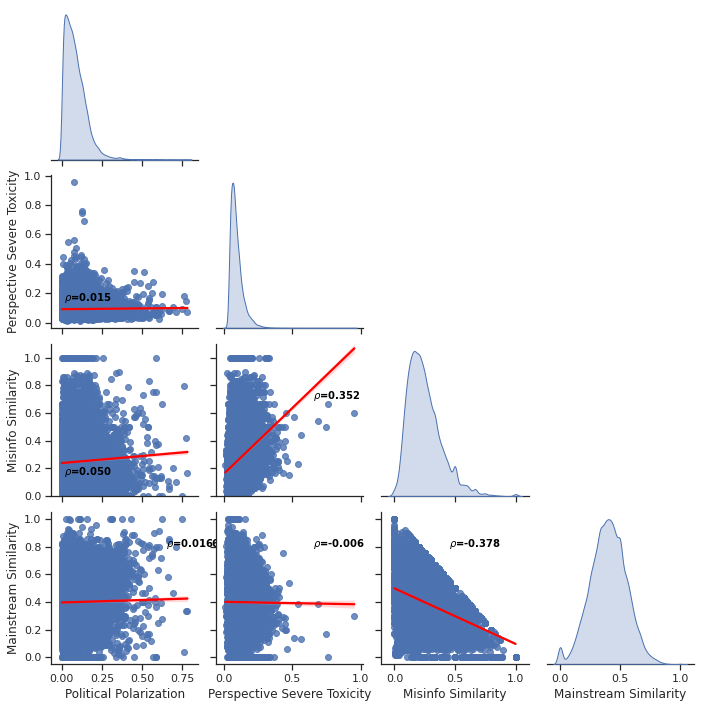
\includegraphics[width=1\columnwidth]{figures/cross_graphs.png} 
\end{minipage}
\begin{minipage}[l]{0.35\textwidth}
\caption{\textbf{Misinformation, toxicity, and political polarization interactions}--- As subreddits increase in misinformation levels, they become more toxic. However, there is not a large correlation between misinformation levels and the political polarization of subreddits. Similarly, we do not see any correlation between political polarization levels and mainstream similarity; nor do we see any correlation with toxicity levels.\label{figure:cross-graph} }
\end{minipage}

\end{figure}


As seen in Figure~\ref{figure:cross-graph}, across all our 46K considered subreddits, we observe that as subreddits become more similar to misinformation and hyperlink to more \textit{misinfo-oriented} domains, their toxicity increases. This largely matches our observation in Section~\ref{sec:toxicity} that misinformation submissions are in general more toxic/uncivil than authentic news submissions. Misinformation levels in general thus appear to be correlated with increased toxicity. We further again surprisingly see in Figure~\ref{figure:cross-graph} that levels of misinformation are not heavily correlated with political polarization. It does not appear that the most politically polarized environments necessarily rely upon misinformation. For example, the most left-leaning subreddits (Table~\ref{table:mostpolitical-subreddits}) that we observed mostly supported US Senator Bernie Sanders and did not necessarily have high misinformation levels. Conversely, we do not see much of a correlation between subreddits with high mainstream similarity and political polarization and toxicity. This again reinforces our results finding that mainstream news does not have higher levels of toxicity and political polarization level from Section~\ref{sec:toxicity} and Section~\ref{sec:polarization}. We thus see again from this analysis that misinformation is indeed correlated with higher toxicity, while authentic news is largely not. 
%\subsection{Reddit Level Interactions}
%Before examining the interaction directly within


\subsection{Summary}
In this section, we found that misinformation on Reddit largely is correlative with and predictive of higher amounts of incivility and toxicity on the platform. Most markedly, we observed that the comments under misinformation submissions are posted at a rate 60\% higher than the comments under authentic news submissions. Further, while we do observe a dichotomy in the political polarization of users that post misinformation and those that comment on misinformation, somewhat surprisingly, we find that misinformation appears across different political environments, with it not being concentrated just in the political extremes. Lastly, looking at how different levels of misinformation correlate with toxicity, we find the more \textit{misinfo-oriented} submissions a given subreddit has, the more toxic/uncivil it is likely to be. 

 